\begin{enumerate}[label=\thesubsection.\arabic*.,ref=\thesubsection.\theenumi]
\numberwithin{equation}{enumi}
\item A unity feedback control system is characterised by the open-loop transfer function
\begin{align}
G(S) = \frac{2(s+1)}{s^3 + ks^2 + 2s +1}
\end{align}
Find the value of the k for which the system oscillates at 2 rad/s.  Verify your result through a program.\\
%
\solution Fig. \ref{fig:ee18btech11030_block} models the equivalent closed loop system. 

\tikzstyle{block} = [draw, fill=blue!20, rectangle, 
    minimum height=0.7cm, minimum width=0.7cm]
\tikzstyle{sum} = [draw, fill=blue!20, circle, node distance=1cm]
\tikzstyle{input} = [coordinate]
\tikzstyle{output} = [coordinate]
\tikzstyle{pinstyle} = [pin edge={to-,thin,black}]

\begin{tikzpicture}[auto, node distance=2.5cm,>=latex']
    % We start by placing the blocks
    \node [input, name=input] {};
    \node [sum, right of=input] (sum) {};
    \node [block, right of=sum] (controller) {G(s)};
    \node [output, right of=controller] (output) {};
    \node [block, below of=controller] (measurements) {H(s) = 1};

    % Once the nodes are placed, connecting them is easy. 
    \draw [draw,->] (input) -- node {$R(s)\  +$} (sum);
    \draw [->] (sum) -- node {$E(s)$} (controller);
    \draw [->] (controller) -- node [name=y] {$Y(s)$}(output);
    \draw [->] (y) |- (measurements);
    \draw [->] (measurements) -| node[pos=0.99] {$-$} 
        node [near end] {$Y_m(s)$} (sum);
\end{tikzpicture}


%
The characteristic equation is
\begin{align}
1 + G(s) &= 0
\\
\implies 1 + \frac{2(s+1)}{s^3 + ks^2 + 2s +1} &= 0
\\
\text{or, } s^3+ks^2+4s+3 &= 0 
\label{eq:eebtech11030_thi_order_ce}
\end{align}
Constructing the routh array for \eqref{eq:eebtech11030_thi_order_ce}
\begin{align}
\mydet{s^3\\s^2\\s^1 \\ s^0}
\mydet{1 & 4 \\ k & 3 \\  \frac{3-4k}{k} & 0\\ 3 & 0} 
\end{align}
For the system to oscillate, poles should lie on the imaginary axis. 

\begin{align}
\implies \frac{3-4k}{k} = 0, \text{ or, }  k = \frac{3}{4}
\end{align}
Substituting in \eqref{eq:eebtech11030_thi_order_ce},
\begin{align} 
s^3+\frac{3}{4}s^2+4s+3 &= 0
\\
\implies  s &= \frac{-3}{4},\pm 2\j
\end{align}
%
The following code verifies the result.
\begin{lstlisting}
codes/ee18btech11030/ee18btech11030.py
\end{lstlisting}

\item Sketch the impulse response of the closed loop system.
\\
\solution The closed loop response
\begin{align}
 G_{m}(s) &= \frac{G(s)}{1+G(s)}=\frac{2(s+1)}{s^3+\frac{3}{4}s^2+4s+3} 
\\
 &= \frac{8}{73(s+\frac{3}{4})}+ \frac{-8s+152}{73(s^2+4)}
\\
 \implies g_{m}(t) &= \frac{8}{73}e^{-\frac{3t}{4}}u(t)- \brak{\frac{8}{73}}\sin\brak{2t} +\brak{\frac{152}{73}}\cos\brak{2t}
\end{align}
%
The following code 
\begin{lstlisting}
codes/ee18btech11030/ee18btech11030_1.py
\end{lstlisting}
plot Fig. \ref{fig:ee18btech11030_sine} .
%
\begin{figure}[!h]
\centering
  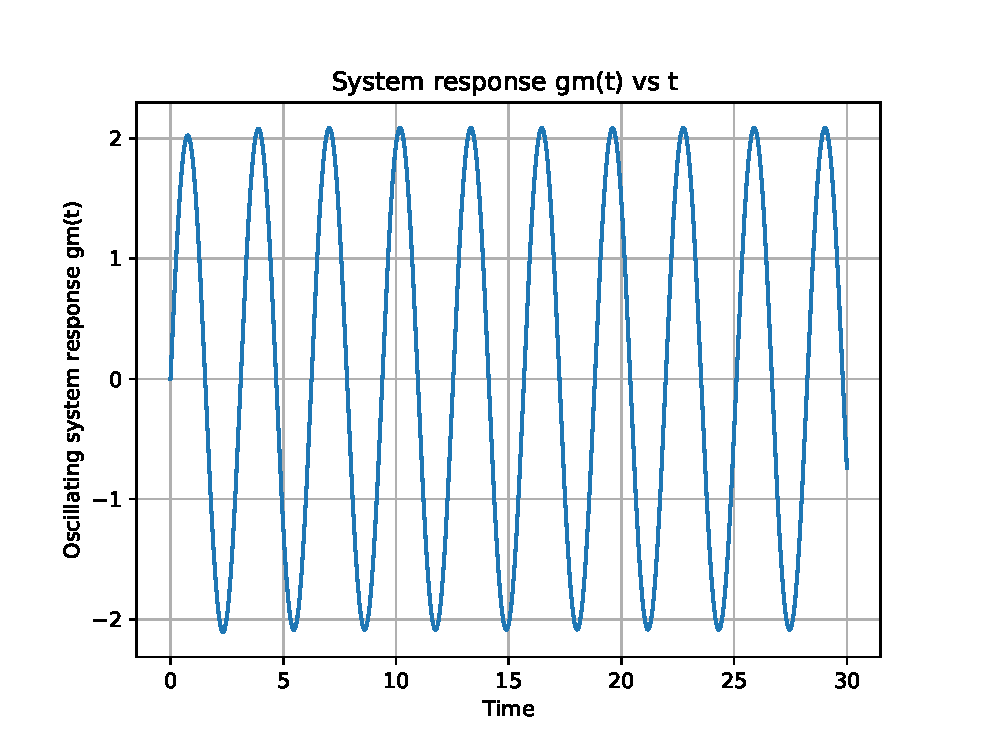
\includegraphics[width=\columnwidth]{./figs/ee18btech11030/ee18btech11030_1.eps}
\caption{}
\label{fig:ee18btech11030_sine} 
\end{figure}
%
This shows that system oscillates at 2 rad/sec.
\end{enumerate}
